\chapter{The simulator}

[This chapter is focused on the simulator implementation]

\section{Data structures}

The simulator is designed for space domains of one or two dimensions. In order 
to parallelize the computation of each step, the space domain is distributed in 
blocks. First the space domain is split in one specific dimension into MPI 
blocks, which will be distributed among each compute node. Communications will 
be needed to share information between MPI blocks.

The second hierarchy splits MPI blocks into task blocks, which can run in 
parallel inside a compute node. Communications are not needed, as we can use 
shared memory in the same compute node.

Inside each task block, we have a small portion of the space domain: the grid 
points of the fields and the particles inside the physical space of the block.  
Additionally, ghost points are placed at the boundaries of the positive 
neighbours in each dimension of the problem.

% TODO; Write about ghost points, and why they are needed

\begin{figure}[h]
	\centering
	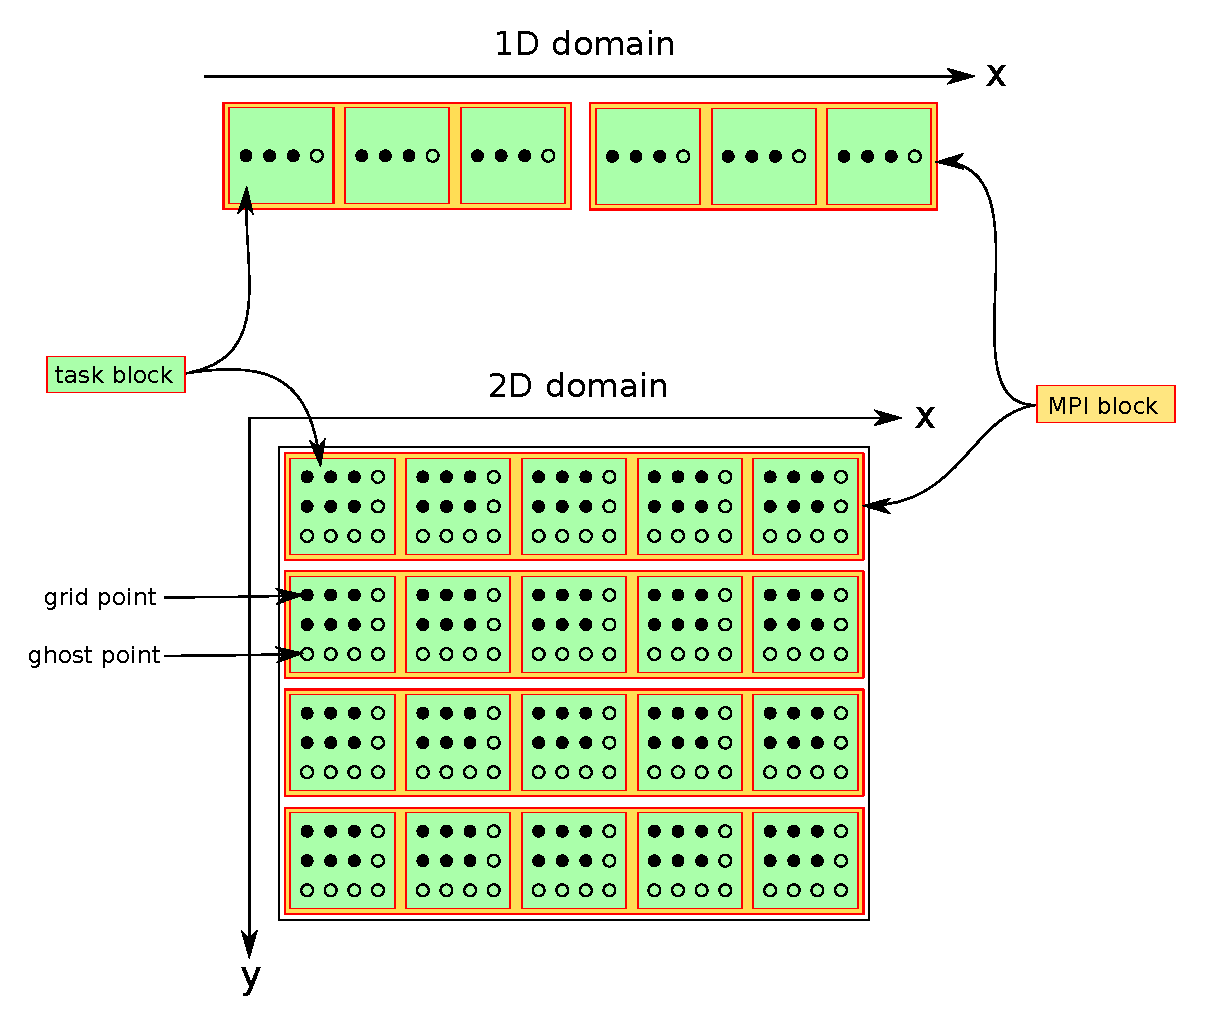
\includegraphics[width=\linewidth]{domain-blocks.pdf}
	\caption{Domain blocks}
	\label{fig:domain-blocks}
\end{figure}

A summary of the data layout can be seen in the figure \ref{fig:domain-blocks}, 
where the physical placement of each block corresponds to the physical position 
of the grid points. The 1D domain has 2 MPI blocks with 3 task blocks each, and 
3 grid points per block with 1 ghost point. In total, the space is discretized 
	in 18 grid points, which require 24 with the ghost points.

Similarly, for 2D the number of ghost points increase, as the frontier now has 2 
dimensions, leading to blocks with 6 grid points and 6 ghost points. The whole 
domain is discretized in 120 grid points, a total of 240 with ghost points.

\section{Simulation flow}

The simulation follows a very precise set of steps to ensure the correct 
behavior of the physical simulation. Three main stages can be easily identified: 
Initialization, loop and finish.

\subsection{Initialization}

The iteration counter is initially set to $-2$, as we are going to do two 
previous phases before the simulation begins:

\paragraph{Allocation phase}
After $P$ processes were created (as in MPI processes), now we create the 
different structures to hold the simulation data. First the fields are 
distributed into task blocks, grouped in each process. For each specie, we 
distribute the particles based on the particle index $p_i$, minimizing the 
difference of the number of particles between blocks. The position, velocity and 
other parameters are set on each particle, independently of the actual block 
they reside.

Once all particles are initialized, we begin to move them to the correct block, 
based on the particle position, and increment the iteration counter. Finally, 
the charge density field $\rho$ is initially computed, as we want the begin the 
simulation with the computation of the electric field E from $\rho$

\paragraph{Rewind phase} The simulation time is not advanced equally for the 
speed and position of the particles. At time $t$ the velocity computed at time 
$t + \dt/2$ whereas the position is computed at time $t$. In order to begin the 
simulation, the velocity of the particles is advanced half time-step backwards 
in time. This extra step is computed at the iteration $i=-1$, as we need the 
iteration counter to be always increasing (as is used in the message exchange as 
unique identifier).

\subsection{Loop}

The loop of the simulation perform four main phases:

\begin{itemize}
\item Solve field equation to get $E$ from $\rho$.
\item Interpolate $E$ at particle positions $E_p$.
\item Particle motion based on $E_p$ and $B_0$.
\item Accumulate charge density $\rho$ at the new position of particles.
\end{itemize}

\subsubsection{Solver}

We use the MFT method to solve the equation:
\begin{equation}
\nabla^2 E = - \frac{\rho}{\epsilon_0}
\end{equation}

\subsection{Finish}

Here we hopefully save some information of the simulation to disk...
